
\subsection{Work Plan, Timeline, and Team} \label{sec:workplan}

% \BfPara{Staged Scope} We stage the program into Phase 1 (Years~1 and~2) and a Phase 2 (Years~3 and~4). Phase 1 targets open and architecturally complementary models on multiple embodiments, and develops ABBP, STAP, and TTDA with related baselines together with the TACD and AGAT defenses and their baselines. 
% The Phase 2 adds emerging models, multimodal analysis, safety and interpretability analysis, and the full public release of VLA-SecBench. 
\autoref{fig:workplan_timeline} summarizes the schedule of the research-plan tasks during the project period.

\begin{figure*}[h]
\centering
\resizebox{0.8\textwidth}{!}{%
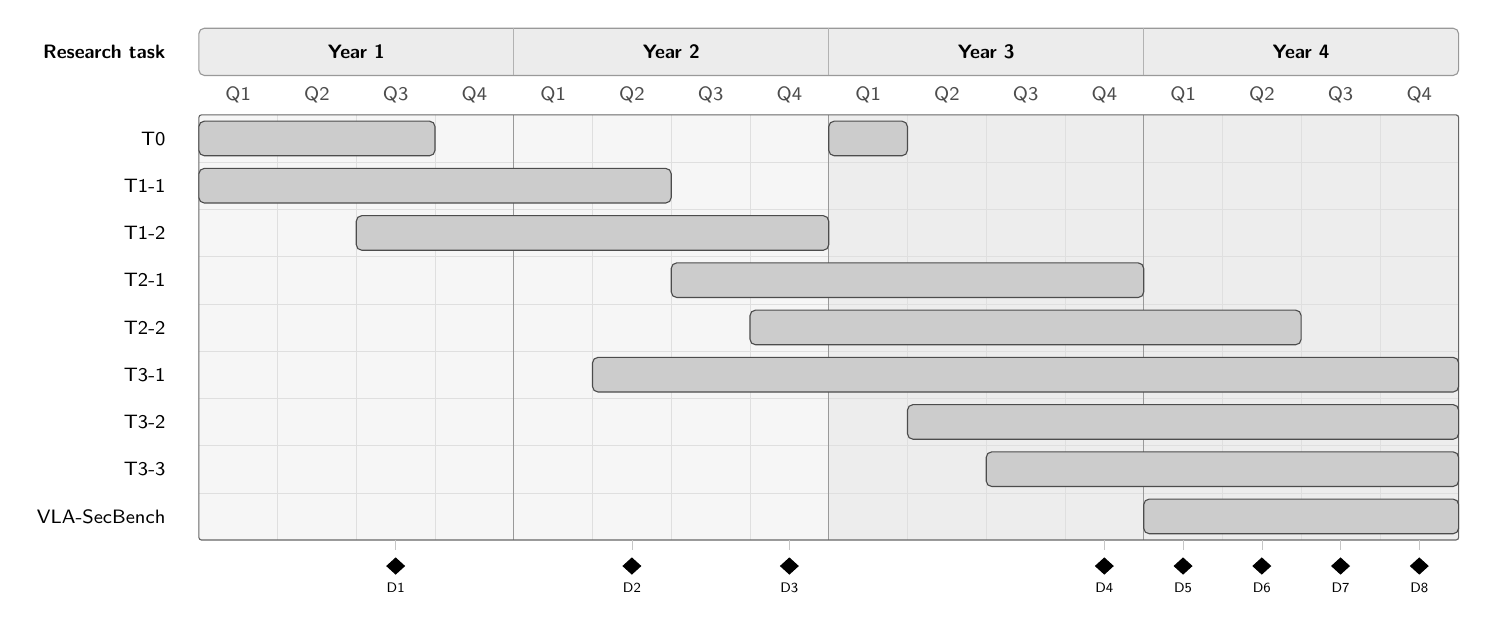
\begin{tikzpicture}[font=\scriptsize\sffamily,
  bar/.style={fill=gray!40, draw=black!70, rounded corners=2pt},
  ]
  %%% activity-band background shading %%%
  \fill[gray!7]  (0,-4.0) rectangle (8,1.4);
  \fill[gray!14] (8,-4.0) rectangle (16,1.4);

  %%% horizontal row separators %%%
  \foreach \hy in {0.80,0.20,-0.40,-1.00,-1.60,-2.20,-2.80,-3.40}
    \draw[very thin, gray!25] (0,\hy) -- (16,\hy);

  %%% vertical quarter gridlines %%%
  \foreach \gx in {1,2,3,5,6,7,9,10,11,13,14,15}
    \draw[very thin, gray!25] (\gx,-4.0) -- (\gx,1.4);
  %%% year boundary lines %%%
  \foreach \gx in {4,8,12}
    \draw[thin, black!40] (\gx,-4.0) -- (\gx,1.4);
  %%% outer chart border %%%
  \draw[black!60, rounded corners=1pt] (0,-4.0) rectangle (16,1.4);

  %%% year header band %%%
  \fill[gray!15, draw=black!40, rounded corners=2pt] (0,1.9) rectangle (16,2.5);
  \foreach \gx in {4,8,12} \draw[black!30] (\gx,1.9) -- (\gx,2.5);
  \node[font=\scriptsize\bfseries\sffamily] at (2,2.2)  {Year 1};
  \node[font=\scriptsize\bfseries\sffamily] at (6,2.2)  {Year 2};
  \node[font=\scriptsize\bfseries\sffamily] at (10,2.2) {Year 3};
  \node[font=\scriptsize\bfseries\sffamily] at (14,2.2) {Year 4};

  %%% quarter tick numbers %%%
  \foreach \g in {1,...,16} {
    \pgfmathtruncatemacro{\qn}{mod(\g-1,4)+1}
    \node[font=\scriptsize\sffamily, text=black!70] at (\g-0.5,1.65) {Q\qn};
  }

  %%% left-hand labels %%%
  \node[anchor=east, font=\scriptsize\bfseries\sffamily] at (-0.3,2.2)  {Research task};
  \node[anchor=east] at (-0.3,1.10)  {T0};
  \node[anchor=east] at (-0.3,0.50)  {T1-1};
  \node[anchor=east] at (-0.3,-0.10) {T1-2};
  \node[anchor=east] at (-0.3,-0.70) {T2-1};
  \node[anchor=east] at (-0.3,-1.30) {T2-2};
  \node[anchor=east] at (-0.3,-1.90) {T3-1};
  \node[anchor=east] at (-0.3,-2.50) {T3-2};
  \node[anchor=east] at (-0.3,-3.10) {T3-3};
  \node[anchor=east] at (-0.3,-3.70) {VLA-SecBench};

  %%% research-task bars (active quarters) %%%
  \fill[bar] (0,0.88)   rectangle (3,1.32);   % T0  Y1Q1-Y1Q3
  \fill[bar] (8,0.88)   rectangle (9,1.32);   % T0  Y3Q1 refresh
  \fill[bar] (0,0.28)   rectangle (6,0.72);   % T1-1 Y1Q1-Y2Q2
  \fill[bar] (2,-0.32)  rectangle (8,0.12);   % T1-2 Y1Q3-Y2Q4
  \fill[bar] (6,-0.92)  rectangle (12,-0.48); % T2-1 Y2Q3-Y3Q4
  \fill[bar] (7,-1.52)  rectangle (14,-1.08); % T2-2 Y2Q4-Y4Q2
  \fill[bar] (5,-2.12)  rectangle (16,-1.68); % T3-1 Y2Q2-Y4Q4
  \fill[bar] (9,-2.72)  rectangle (16,-2.28); % T3-2 Y3Q2-Y4Q4
  \fill[bar] (10,-3.32) rectangle (16,-2.88); % T3-3 Y3Q3-Y4Q4
  \fill[bar] (12,-3.92) rectangle (16,-3.48); % Benchmark Y4Q1-Y4Q4

  %%% deliverable markers along the bottom axis %%%
  \foreach \mx/\ml in {2.5/D1, 5.5/D2, 7.5/D3, 11.5/D4, 12.5/D5, 13.5/D6, 14.5/D7, 15.5/D8} {
    \draw[very thin, gray!45] (\mx,-4.0) -- (\mx,-4.13);
    \fill[black, draw=black] (\mx,-4.23) -- (\mx-0.11,-4.33) -- (\mx,-4.43) -- (\mx+0.11,-4.33) -- cycle;
    \node[font=\tiny\sffamily, anchor=north, inner sep=1pt] at (\mx,-4.5) {\ml};
  }
\end{tikzpicture}%
}\vspace{-2ex}
\caption{Work-plan timeline with anticipated project start on (May~2027): Year~1 (May~2027--Apr~2028) to Year~4 (May~2030--Apr~2031). Quarters marked as Q1--Q4 and deliverables as D1--D8. {\textbf{Deliverables:} \textbf{D1} model and data repository with reproducible baselines (Y1Q3); \textbf{D2} ABBP with evasion and poisoning variants (Y2Q2); \textbf{D3} STAP and TTDA with open-source attack release (Y2Q4); \textbf{D4} TACD and AGAT with open-source defense release (Y3Q4); \textbf{D5} cross-model, cross-embodiment transferability matrix (Y4Q1); \textbf{D6} safety benchmark across models, embodiments, and tasks (Y4Q2); \textbf{D7} multimodal attack and defense evaluation (Y4Q3); \textbf{D8} VLA-SecBench v1.0 and the action-interpretability toolkit publicly released (Y4Q4).}}
\label{fig:workplan_timeline}
\end{figure*}